\section{Analyse et conception d'un flip flop D}
On souhaite réaliser un flip flop D dont le symbole est le suivant :
\begin{figure}[h!]
    \begin{center}
        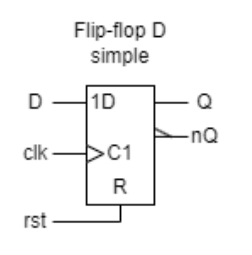
\includegraphics[scale=0.75]{images/Symboles/flipflopD.png}
    \end{center}
    \caption{Symbole du flip flop D}
\end{figure}
\newline
La table des fonctions synchrones est la suivante :
\begin{table}[h!]
    \begin{center}
        \begin{tabular}{|c|c|}
        \hline
        \textbf{D} & \textbf{Q+} \\
        \hline
        0 & 0\\
        \hline  
        1 & 1 \\
        \hline
        \end{tabular}
    \end{center}    
    \caption{Table de vérité du flip flop D}
\end{table}
\newline
La sortie nQ est simplement l'inverse de Q.
\subsection{Description VHDL}
On dispose de l'entité suivante: 
\begin{verbatim}
entity dff_ar is
   port( 
      Rst_i   : in    std_logic;
      Clk_i   : in    std_logic;
      D_i     : in    std_logic;
      Q_o     : out   std_logic;
      nQ_o    : out   std_logic
   );
end dff_ar ;    
\end{verbatim}
Selon  la méthodologie du cours, nous devons avoir deux signaux internes :
\begin{verbatim}
    signal D_s : std_logic; 
    signal Q_s : std_logic; 
\end{verbatim}
Puis nous avons la logique suivante:
\begin{verbatim}
    D_s <= D_i; -- Décodeur d'états présent
  
  -- Process de bascule
   process(reset_i, Clk_i)
   begin
      if reset_i = '1' then
      Q_s <= '0'; --Etat par défaut
      elsif rising_edge(Clk_i) then
      Q_s <= D_s;
      end if;
   end process;
 
\end{verbatim}
On affiche ensuite les sorties:
\begin{verbatim}
  -- Sorties
   Q_o <= Q_s;
   nQ_o <= not(Q_s);
\end{verbatim}
La description complète du flip flop D est disponible dans le fichier \textit{src/dff\_ar.vhd}.
\subsection{Simulation Automatique}
\begin{verbatim}
-- Loading package STANDARD
# -- Loading package TEXTIO
# -- Loading package std_logic_1164
# -- Compiling entity dff_ar_tb
# -- Compiling architecture test_bench of dff_ar_tb
# -- Loading entity dff_ar
# ** Warning: ../src_tb/dff_ar_tb.vhd(51): (vcom-1236) Shared variables must be of a protected type.
# End time: 10:54:06 on Apr 15,2026, Elapsed time: 0:00:01
# Errors: 0, Warnings: 1
# End time: 10:54:07 on Apr 15,2026, Elapsed time: 0:03:22
# Errors: 1, Warnings: 0
# vsim -voptargs=""+acc"" work.dff_ar_tb 
# Start time: 10:54:07 on Apr 15,2026
# ** Note: (vsim-3812) Design is being optimized...
# Loading std.standard
# Loading std.textio(body)
# Loading ieee.std_logic_1164(body)
# Loading work.dff_ar_tb(test_bench)#1
# Loading work.dff_ar(comport)#1
run -all
# ** Note: >> Debut de la simulation
#    Time: 0 ns  Iteration: 0  Instance: /dff_ar_tb
# ** Note: >>Nombre d'erreur détectée = 0
#    Time: 552 ns  Iteration: 0  Instance: /dff_ar_tb
# ** Note: >>Fin de la simulation
#    Time: 552 ns  Iteration: 0  Instance: /dff_ar_tb
\end{verbatim}
\subsection{Vue RTL}
\begin{figure}[h!]
    \begin{center}
        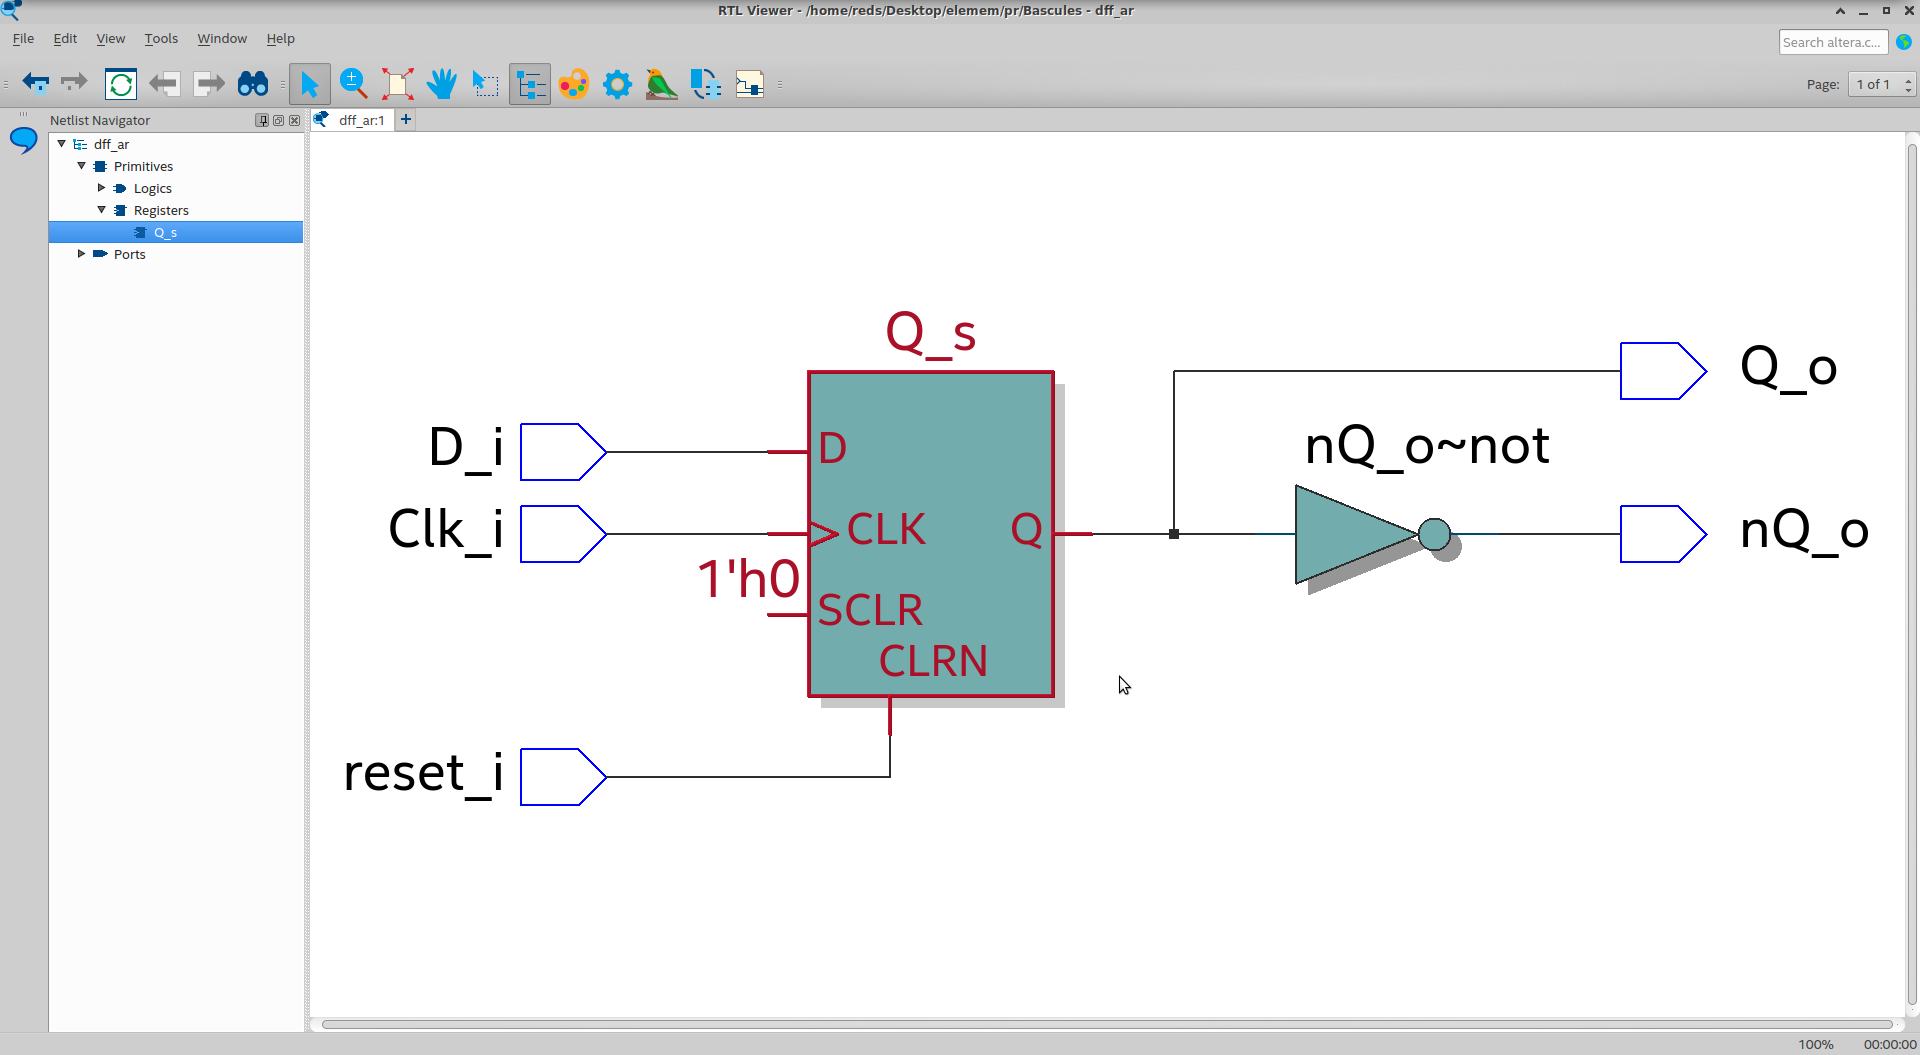
\includegraphics[scale=0.2]{images/VueRTL/VueRTLdffar.png}
    \end{center}
    \caption{Vue RTL du flip flop D}
\end{figure}
On voit clairement la bascule D, et la porte NOT pour la sortie nQ.
